\documentclass[a4paper,11pt]{report}

\usepackage{times}
\usepackage{natbib}
\usepackage[pdftex]{graphicx}
\usepackage{epstopdf}
\usepackage{algorithm}
\usepackage{algorithmic}

\title{Using Competence Models in Active Learning}
\author{Charles McCarthy\\
  106380221\\
  \texttt{cmmc1@student.cs.ucc.ie}
  \\Supervisor: Dr. Derek Bridge}
\date{March 2012}

\begin{document}

\maketitle

\begin{abstract}
An overview of the fundamental concepts in Active Learning, with particular focus on the use of Competence Models. Experimental analysis of basic Selection Strategy approaches, along with experiment on new Competence Model based approaches.
\end{abstract}

\chapter*{Declaration of Originality}
\vspace*{\fill}
In signing this declaration, you are confirming, in writing, that the submitted work is your own original work, unless clearly indicated otherwise, in which case, it has been fully and properly acknowledged.

I hereby declare that:
\begin{itemize}
	\item this is all my own work, unless clearly indicated otherwise, with full and proper accreditation;
	\item with respect to my own work: none of it has been submitted at any educational institution contributing in any way towards an educational award;
	\item with respect to another's work: all text, diagrams, code, or ideas, whether verbatim, paraphrased or otherwise modified or adapted, have been duly attributed to the source in a scholarly manner, whether from books, papers, lecture notes or any other student's work, whether published or unpublished, electronically or in print. 
\end{itemize}

\vspace{\stretch{1.0}}
{
\renewcommand{\arraystretch}{4.5}
\begin{center}
 	\begin{tabular}{l @{:} p{0.4in} l}
		Name & & Charles McCarthy \\
		Signature & & \makebox[2.5in]{\hrulefill} \\
		Date & & March 2012 \\
	\end{tabular}
\end{center}
}
\vspace{\fill}





\tableofcontents

\chapter{Introduction}
\section{Active Learning Overview}
The key concept of Active Learning is that a machine learning program has a say in its own learning process, by being capable of choosing the data from which it learns. 

This concept fits particularly well in the domain of Case Based Systems. In Case Based Systems, the system has a pool of 'cases' for which it knows the label. When an unlabelled case is presented to the system, the system uses this pool to try to guess the label of the unlabelled case.

The facet of Active Learning we will subsequently consider is based on the idea that there is a large quantity of unlabelled cases available, but getting labels (or more likely, consulting a human oracle) is an expensive process, for which it is undesirable to apply to the entire unlabelled set. The aim for the system is to choose a subset of these unlabelled cases for which to request a label. These are then used as the system's pool of labelled cases which it will consult in future.

The system would like to maximize its classification accuracy for future instances, but have to resort to asking the expert external to the system for a minimal number of labels.

For an in-depth review of Active Learning, and some of the recent Active Learning literature, consult \citep{Settles2010}


\section{Importance of Active Learning}
There are many real-world domains in which a large quantity of unlabelled data is available, but the process of manually labelling all of that data is not feasible. 

A human expert is often needed to label instances of the data. This human factor limits the quantity of data which can be labelled. The financial cost can be significant, and the availability of such an expert can also be a limiting factor.

Often - the 'expert' labelling process is in itself exceedingly slow compared to either the amount of unlabelled data available, or the rate at which new data is being generated. 

Machine Learning seems a clear answer for these type of scenarios, but for Machine Learning, one still needs training instances to initially train the system.

\subsection{Examples of Active Learning Domains}
\subsubsection{Recommendation Engines}
In recommendation engines, the user can be thought of as the "expert". It is based on their feedback (either implicit or explicit) that the recommendation engine can know if an item was relevant to the user or not. It is likely that there is a vast library from which a recommendation can come, but the quantity of user feedback may be limited.

What is sometimes done in these systems is that the engine includes some results it is relatively certain will be relevant to the user, but others of which it is uncertain, but would like to gain feedback on from the user. Only comparatively few of these instances can be given to the user for feedback, as doing otherwise would negatively impact the user's experience.

Choosing which uncertain instances to present to the user to maximize the system's competence-gain is therefore an important problem for the system.

\subsubsection{Medical Data}
Medical data is another area in which Active Learning is of particular interest and relevance.

Vast quantities of patient data exists, but each patient data instance is unlikely to have results of tests for every possible disease / condition. It is obviously preferable though to detect any illness or condition a person has as soon as possible, so that appropriate measures are taken. It is not feasible however to test each individual for every possible illness.

When building a system to predict illnesses, one would want to minimize the number of physical tests to be carried out on patients for the purpose of training the system. It is in this way that Active Learning can have a useful role to play.

\subsubsection{Computer Vision}
Computer Vision is another area in which large quantities of data are available, and easy to generate, but manual labelling is incredibly tedious.

\subsubsection{Text Classification}
Increasingly with the proliferation of the internet, and in particular social media, text classification has many practical applications. The traditional example is that of email spam analysis, but more and more, sentiment analysis is becoming an active area of interest.

Vast quantities of textual data are often available for the target domain, though initial labelling requires human involvement. Active Learning thus has a potentially very useful role in the process, helping in maximising the system gain with the minimum of data.

\subsubsection{Voice Analysis}

Speech recognition is one area that can bring immense benefit to users, but for which manual labelling requires expert skills, and is painstakingly slow even with a trained expert's involvement. For such systems, it is highly desirable to reduce the quantity of data that must be manually labelled to bring the system to an acceptable rate.

Other forms of voice analysis can also potentially benefit from active learning approaches - e.g. Sentiment Analysis.

\section{Fundamental Concepts}
\subsection{Case Base}
The Case Base is the labelled pool of data which the overall system consults when a new unlabelled instance is presented for classification.

While not essential, a kNN approach fits the Case Base concept quite well.

\subsection{Oracle/Expert}
The Oracle (or Expert) is the entity which the system may consult if it wishes to determine the true label for an instance.

Often, the Expert is a human familiar with the domain who must manually classify the instance. Though the Expert may also just be another system, but for which there is some expense in using to determine a class. \footnote{Here, we use the word "expense" in its broadest possible meaning. It may be financially expensive, computationally expensive, or simply take an exceedingly long amount of time to run. In any event, "expense" refers to some undesirable operation for which we want to minimise the number of calls.}

\subsection{Selection Strategy}
While the term Selection Strategy can have slightly different meanings given the type of Active Learning being considered, we will subsequently use the phrase to mean the algorithmic approach taken to determine which unlabelled instances to query with the Oracle for the true label.

\subsection{Stopping Condition}
The Stopping Condition of the system is the point at which the system must stop consulting the Oracle.

\subsubsection{Examples of stopping conditions}
\paragraph{Oracle Budget} 
The Oracle is willing to classify only a fixed number of instances.

\paragraph{Desired Classification Accuracy} 
The system stops asking the Oracle for classifications after it is capable of achieving a certain classification accuracy on its test set.

\section{Variations / Related Areas}
Many variations on the concept of Active Learning exist. The following it intended to give just a small subset of examples, as opposed to an exhaustive listing.

\subsection{Case Base Maintenance}
Case Base Maintenance is concerned with the task of how to maintain a case base. 

Over time, as new instances are added, the case base size increases. This can have an adverse effect on system performance, thus it can be desirable to have the case base be as minimal as possible, while maintaining classification accuracy.

Another consideration is that some cases may be adversely affecting the system's classification accuracy. It may be that these instances were initially misclassified by the 'expert', the underlying data was noisy, or it could be that the nature of the domain has changed and that similar instances now actually have a different label. The detection of these cases is therefore an important part to long-running Case Based Systems.

Overall, Case Base Maintenance can be summarised as the process of maintaining a case base to a desirable level over time.

\subsection{Stream Based Learning}
In this methodology, the system does not just select at the outset from an unlabelled pool the instances to request classification by the Expert. Instead, It is presented with a stream of instances, and for each instance, it may either itself guess the classification (if it is relatively sure it is correct), or it may defer the decision to the Expert.

This notion can sometimes be more useful - but it is unlikely in practice that the system would query at any arbitrary time for an expert classification, since with the usual case of requiring human involvement, the expert may not be available at all times.

What is more likely is that the system would keep note of instances it is very unsure of, guess the classification anyway if an immediate response is required, and at the next opportunity, query the oracle in batch regarding the true classification.

\subsection{Batch Learning}



\subsection{Noisy Oracle}
\subsection{Classification Cost Variation}
This paper does not deal with instance classification cost variation, instead assuming a fixed cost.

\subsection{Case Interdependence}

\section{Project outline}

\chapter{Literature Review}

\section{Common Concepts}
Certain concepts very frequently occur in the Active Learning Literature, so these will be outlined first.

\subsection{Similarity/Distance}
\subsection{Density}
\subsection{Diversity}
\subsection{Solves / Classifies / Contributes}
Make note of the different definitions.
\subsection{Clustering}

\chapter{Platform Architecture}
\section{Overview}
- Python, orange, Weka initially investigated. Intended for evaluating Selection Strategies.

\section{Selection Strategy Evaluation}

\section{Core Classes}
\subsection{k Nearest Neighbour Functionality}
\section{Inputs}
\subsection{Data Files}
\subsubsection{Orange Supported}

\subsubsection{Custom Pre-computed distance Format}

(Also note - for compression, and due to text based method used as opposed to binary. This format was chosen for ease of human readability and given that the datasets we use are relatively small).

\subsection{Experiment Definitions}

\section{Experiment Running}
- give basic algorithm in SelectionStrategyEvaluator.
\section{Outputs}
(Initially used matplotlib - but non pythonic, etc.)
\chapter{Competence Models}
\section{Overview}
\section{Fundamentals}
\subsection{Classifies / Misclassifies}
\subsubsection{Case Contribution\label{sec:contributes}}
Both Classifies and Misclassifies are subsequently defined in terms of \emph{Case Contribution}.

A case $c$ contributes to another case $c\prime$'s classification if $c$ is retrieved as a nearest neighbour of $c\prime$ and $c$ aids 'positively' to $c\prime$'s classification (i.e. is the same class as $c\prime$ if $c\prime$ is correctly, or is a different class to  $c\prime$ if  $c\prime$ is incorrectly classified).
\subsubsection{Classifies}
\begin{quote}
$ Classifies(t, c) $ means that case c contributes to the correct classification of target case t. This means that target case t is successfully classified and case c is returned as a nearest neighbour of case t and has the same classification as case t.
\end{quote}
\citet{Delany2009}

Therefore, for $ Classifies(t, c) $:
\begin{enumerate}
	\item t must be correctly classified by the case base.
	\item c must be returned as a NN of t in that correct classification.
	\item c must be of the same class as t.
\end{enumerate}

\subsubsection{Misclassifies}

\begin{quote}
$ Misclassifies(t, c ) $ means that case c contributes in some way to the incorrect classification of target case t. In effect this means that when target case t is misclassified by the case-base, case c is returned as a neighbour of t but has a different classification to case t.
\end{quote}
\citet{Delany2009}

Therefore, for $ Misclassifies(t, c) $:
\begin{enumerate}
	\item t must be incorrectly classified by the case base.
	\item c must be returned as a NN of t in that classification.
	\item c must be of a different class than t's actual class.
\end{enumerate}

\subsubsection{Example}
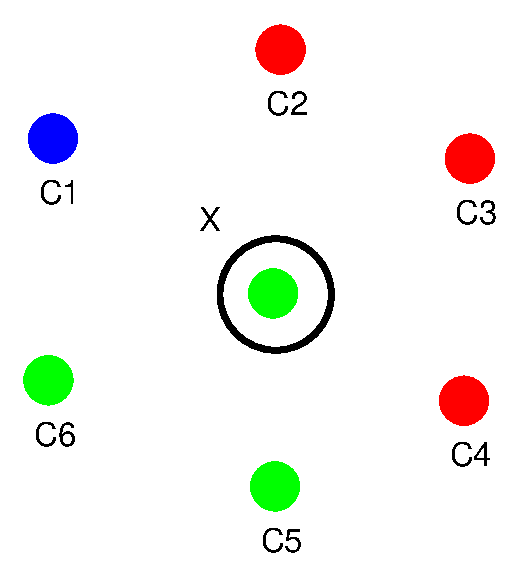
\includegraphics[width=5cm]{EqualDistanceMisclassifiesEg}

e.g  in the above example, the circled case 'x' is incorrectly classified as red by the case base (with k=6). Here, the 3 reds (c2, c3 and c4) and the 1 blue (c1) contribute to the incorrect classification, and thus:
\begin{itemize}
	\item $ Misclassifies(x, c1) $
	\item $ Misclassifies(x, c2) $
	\item $ Misclassifies(x, c3) $
	\item $ Misclassifies(x, c4) $
\end{itemize}

\subsection{Nearest Neighbours / Reverse Nearest Neighbours}
Before considering the definitions of the RCDL sets, it is useful to consider the notion of nearest neighbours and reverse nearest neighbours, so that the RCDL sets can be framed in those terms.

\subsubsection{Nearest Neighbours (NNs)}
For a case c, $ NNs(c) $ is the set of cases within the k nearest neighbours of c, excluding c itself.

\subsubsection{Reverse Nearest Neighbours (rNNs)}
For a case c, $ rNNs(c) $ is the set of cases that have c in their NNs set.

\subsubsection{Example}
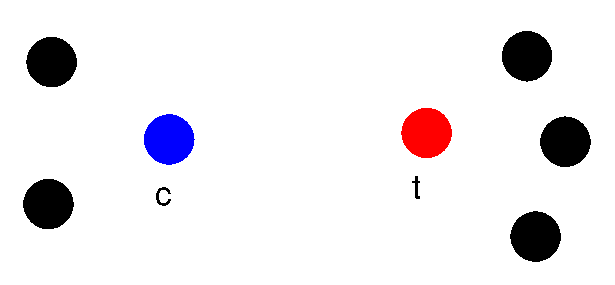
\includegraphics[width=5cm]{RcdlNnRnnEg}

For $k=3$:
\begin{itemize}
	\item $ t \in NNs(c) $
	\item $ c \in rNNs(t) $
\end{itemize}

\subsection{RCDL Definitions}
Overall Reachability and Coverage relate to cases being correctly classified by the case base, whereas Dissimilarity and Liability relate to cases being incorrectly classified by the case base.

Reachability and Dissimilarity are concerned with the neighbouring cases of a case, whereas Coverage and Liability are concerned with the cases to which a case is a neighbour.

\subsubsection{Reachability Set}
\[ ReachabilitySet(c \in C) = \left\lbrace t \in C : Classifies(c, t) \right\rbrace \] \cite{Delany2009}
If c is correctly classified by the case base, these are all the cases in $ NNs(c) $ that have the same class as c. Otherwise, this set is empty (and the Dissimilarity set is instead populated).

\subsubsection{Coverage Set}
\[ CoverageSet(c \in C) = \left\lbrace t \in C : Classifies(t, c) \right\rbrace \]
These are all the cases $ t \in rNNs(c) $ such that t is correctly classified by the case base and the class of t is the same as the class of c.

\subsubsection{Dissimilarity Set}
\[ DissimilaritySet(c \in C) = \left\lbrace t \in C : Misclassifies(c, t) \right\rbrace \]  \cite{Delany2009}
If c is incorrectly classified by the case base, these are all the cases in $ NNs(c) $ that have a different class than the actual class of c. Otherwise, this set is empty (and the reachability set is instead populated).

\subsubsection{Liability Set}
\[ LiabilitySet(c \in C) = \left\lbrace t \in C : Misclassifies(t, c) \right\rbrace \]  \cite{Delany2009}
These are all the cases $ t \in rNNs(c) $ such that t is incorrectly classified by the case base, and the class of c is different from the class of t.

\section{RCDL Consequences}

\subsection{Either-or nature of Reachability and Dissimilarity Sets}
If a case has a non empty reachability set then it has been classified correctly by the case-base and, as such, will have an empty dissimilarity set and vice versa.

Intuitively – these sets simply represent the set of cases that are 'responsible' for / contribute to a case's classification (with the notion of 'contributes' as outlined above on page \pageref{sec:contributes}). 

If the case is correctly classified, this set is said to be the Reachability set, whereas if incorrectly classified, it is termed the Dissimilarity set.

\subsection{Reachability-Coverage / Liability-Dissimilarity Duality}
Simply put, if case $c$ occurs in case $t$'s Reachability set, case $t$ occurs in $c$'s Coverage set. Similarly with Liability and Dissimilarity.
The reasoning is as follows:
\begin{itemize}
	\item Take a single case pair, $c1$ and $c2$ such that $Classifies(c1, c2)$.
	\begin{itemize}
		\item $c2$ contributes to the correct classification of $c1$.
	\end{itemize}
	\item From $c2$'s perspective, $c1$ is in its Coverage set.
	\begin{itemize}
		\item From the formula above, from $c2$'s perspective, $c=c2$, and $t=c1$, and it is the case that $Classifies(t, c)$.
	\end{itemize}
	\item From $c1$'s perspective, $c2$ is in its Reachability set.
	\begin{itemize}
		\item From the formula above, from $c1$'s perspective, $c=c1$ and $t=c2$, and it is the case that $Classifies(t, c)$.
	\end{itemize}
\end{itemize}

Similar reasoning can be applied to the Liability and Dissimilarity sets.

This point is easier to understand just by intuition around the plain-English definitions of the RCDL profiles above.

\subsection{Reachability is to Dissimilarity as Coverage is to Liability}
This is obvious from looking at the formulas, but is worth pointing out for future notes.

\subsection{Reachability/Dissimilarity concerned with Nearest Neighbours, Coverage/Liability with Reverse Nearest Neighbours \label{sec:RdWithNnClWithRnn}}
This can simply be derived through the definitions above, but of primary note is that:
\begin{itemize}
	\item The Reachability and Dissimilarity of a case can be inferred by just looking at that case's nearest neighbours
	\item The Coverage and Liability of a case can be inferred by just looking at that case's reverse nearest neighbours (assuming the case-base classification of each of the reverse nearest neighbours is known)
\end{itemize}

\subsection{Max Size of Reachability and Dissimilarity Sets bounded to K}
Given that the Reachability and Dissimilarity of a case are always subsets of that case's NNs, the maximum size is the size of the NNs set – K. (This is assuming that a 'strict' kNN is used, where at max k neighbours are used even when ties exist).

\section{An Incremental Strategy to RCDL}
\subsection{Justification}
For developing new Competence-based Selection Strategies, it would be useful to be able to determine what RCDL changes would occur in the RCDL profiles if a new case was added with a given class. If this were to be done for each unlabelled case when selecting a case to add to the case base, it would be very expensive to re-build the entire set of RCDL profiles for the case base each time.

Thus, an incremental strategy, in which the changes can also be inferred in linear time before actually 'adding' a case, would be very useful.

\subsection{Desired Algorithm Structure}
\subsubsection{Inputs}
\begin{itemize}
	\item A case base 
	\item k – the size of the neighbourhood
	\item RCDL, NN, and rNN profiles for each of the cases
\end{itemize}

For the remainder of this algorithm description, the term 'profile' is used to denote the RCDL profile plus NNs plus rNNs. i.e. 
\begin{verbatim}
CaseProfile:  
  Reachability Set:  {…}
  Coverage Set:      {…}
  Dissimilarity Set: {…}
  Liability Set:     {…}
  NNs:               {…}
  rNNs:              {…}
\end{verbatim}

\subsubsection{Operations}
\paragraph{$Suppose(unlabelled\_case, class)$}
This operation should determine what changes would occur to the profiles of the cases in the case base if a given unlabelled case was added to the case base, with a given class.

A Change to a given case may be denoted as the pair (Added, Removed), where Added and Removed in turn are simply partial profiles. i.e.
\begin{verbatim}
Change:
  Added:
    Reachability Set:  {…}
    Coverage Set:      {…}
    Dissimilarity Set: {…}
    Liability Set:     {…}
    NNs:               {…}
    rNNs:              {…}
  Removed:
    Reachability Set:  {…}
    Coverage Set:      {…}
    Dissimilarity Set: {…}
    Liability Set:     {…}
    NNs:               {…}
    rNNs:              {…}
\end{verbatim}

The output for this algorithm will be a set of (Case, Change) pairs. For algorithmic ease, this also include the input unlabelled case, since technically, adding it will cause cases to be added to its Reachability Set, etc. But understandably, for the input case's Change, the Removed data will always be empty.

\paragraph{$Add(labelled\_case)$}
This operation simply adds a given case to the case base, updating the case base's profiles as appropriate. Operationally, this involves supposing that the case was added with its class using the previous Suppose operation, and updating the case base's profiles as per the returned set of (case, Change) pairs.

\subsection{Algorithm Outline}
The rough approach taken is to first determine the changes which occurred to NNs and rNNs. From these, along with knowledge of the existing RCDL profiles, the changes to Reachability, Coverage, Dissimilarity and Liability are inferred. \footnote{Note – for clarity, the outline refers to updating the actual Case Base Profiles set, whereas really it's a Change object for each one that it modifies, and finally returns}

\subsubsection{Figuring out NN / rNN changes}
\paragraph{Notes}
\subparagraph{Determining if an existing case has the new case as a NN within k}
Unfortunately, each case in the case base needs to be examined to determine if it has the new case as a NN. But because we have the NNs stored for each case in the case base, the examination of each case can be a relatively quick operation (versus the alternative of having to, for each case, go through the entire case base to find its NNs if they weren't stored).

The maximum NN distance in the cached NN list need only be compared to the distance of the new case (with consideration for tie breaking as in the kNN classifier if they're equal).

\subparagraph{Get or create Change in all\_changes for x}
This is simply a shorthand for first checking if there already is a change in all\_changes for 'x', and if so, retrieving it – otherwise creating a new blank Change in all\_changes for 'x', and returning the new Change.

\subparagraph{Duality of NN/rNN changes (both added and removed)}
If a case has a Nearest Neighbour added, then for that Nearest Neighbour, it will get a Reversed Nearest Neighbour added. Thus, for any NN add, there is a corresponding rNN add. Similarly for remove.


\paragraph{Algorithm}

\begin{verbatim}
Figure out the new case's NNs, and for each NN, add the new case to their rNNs
Figure out the existing cases that would have the new case as a NN, and for each:
  Add the existing case to the new case's rNNs
  Add the new case to the existing case's NNs.
  If the new case 'shunted' is an NN of the existing case:
    Remove the shunted case from the existing case's NNs
    Remove the existing case from the shunted case's rNNs.
\end{verbatim}

\subsubsection{Using NN / rNN changes to determine RCDL changes}
\paragraph{Notes}
\subparagraph{Ability to just look at NN changes}
Due to the NN/rNN Duality property described above with regards NN changes, any NN add is guaranteed to have an rNN add, and similarly with remove. This allows us to consider only NN changes, and while dealing with the NN change, deal with the corresponding rNN change.

\subparagraph{Permutations of NN changes}
Because of the previous note, we only really need to deal with the added and removed nearest neighbours. So – the permutations of NN changes for a single case, following 'supposing' the addition of a single case:

\begin{tabular}{ | c | c | p{5cm} |}
	NN Added & NN Removed & Notes \\ \hline
	1 & 1 & Will be the only type when the size of the case base is greater than or equal to  k. \\ \hline
	1 & 0 & Happens only at start, as the NN is filling to capacity. Same as added above. \\ \hline
	0 & 1 & Can never actually happen - would have to be another replace it. \\ \hline
	0 & 0 & Uninteresting - its rNNs will be covered elsewhere with the NN changes of another case. \\ \hline
\end{tabular}

\subparagraph{A NN Removal Guarantees an NN Add} \footnote{in the case of Supposing a case is added}
This can be seen in the truth table above. Because we're only dealing with a new case being added, the effect of the new case can never cause a NN removal without causing a corresponding NN add of the new case. (Because of having a shorter distance to the target case than the furthest-distance NN, the new case will have 'shunted' that NN – causing a NN removal).

This allows us to not worry about, at the stage of dealing with NN removals, if the removal caused the class to change, because we'll be dealing with that scenario anyway in the corresponding add.

\subparagraph{A NN removal might affect R/D of me, C/L of other}
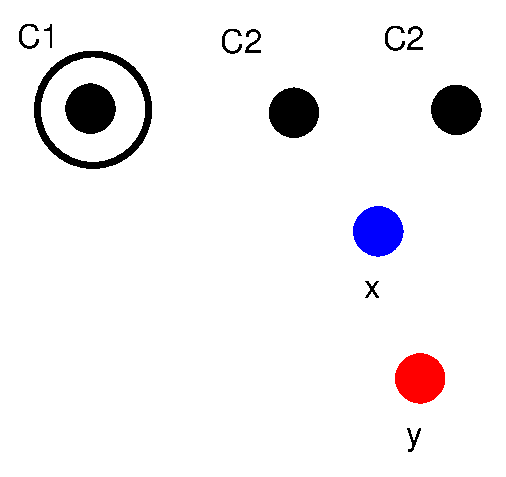
\includegraphics[width=5cm]{NnMightAffectEg}

In the above example,
\begin{itemize}
	\item $k=3$, 
	\item $x$ is the case of interest whose NNs  we'll talk about
	\item $y$ is the new case added to the case base
	\item $c1$, $c2$, $c3$ are the NNs of $x$ prior to $y$ being added
	\item $c1$ is the 'shunted' case which is removed from NNs(x) after $y$ is added.
\end{itemize}

$c1$ was an NN of $x$, and $x$ was an rNN of $c1$. As described previously in \ref{sec:RdWithNnClWithRnn}, a case's NNs can affect its Reachability / Dissimilarity sets, whereas a case's rNNs can affect its Coverage / Liability sets. So the removal of $c1$ as an NN of $x$ (and the corresponding removal of $x$ as an rNN of $c1$) might affect $c1$'s Reachability / Dissimilarity set, and $x$'s Coverage / Liability set, because when $c1$ is removed as a NN, it can't contribute either positively or negatively any more to $x$'s classification.\footnote{Note that it is not guaranteed that $c1$ was in $x$'s Reachability / Dissimilarity set, or that, equivalently, $x$ was in $c1$'s Coverage / Liability set. The sets will only be affected if $c1$ was a 'contributor' of $x$'s classification by the case base. Hence the usage of "might affect".}

All this leads to a simple way to dealing with an NN removal \footnote{The corresponding NN addition will be dealt with separately}:
\begin{itemize}
	\item If $c1$ was in $x$'s Coverage / Liability set, it should be removed.
	\item If $x$ was in $c1$'s Reachability / Dissimilarity set, it should be removed.
\end{itemize}

\subparagraph{Calculating a case's new classification}
This can be done semi-intelligently since a case's old NNs are known. Instead of doing kNN classification with the entire case base, we only need to look at a case's new NNs (which can be inferred from its old NNs and the NN changes) to determine the new classification.

\subparagraph{Correct-classification-status}
We will furthermore commonly talk about a case's correct-classification-status as opposed to its classification alone. It simply means whether a case has been correctly classified by the case base or not. 

\subparagraph{A case's correct-classification-status determining Reachability/Dissimilarity}
If a case is correctly classified by the case base, its Reachability set will be populated. If it is incorrectly classified, its Dissimilarity set will be populated.
 
\subparagraph{Effect of a correct-classification-status changing}
Firstly, we need only worry about if the correct-classification-status of a case changes with the addition of a new case, as opposed to if the classification alone changes.

E.g. if a case's actual class was 'green', it was previously classified 'blue', and with the addition of the new case, it's classified 'red', it has still been incorrectly classified both before and after the addition of the new case, therefore we do not need to worry about scrubbing.

If however the correct-classification-status of a case does change, we need to perform 'scrubbing ' on some of the RCDL sets.

If it went from correctly classified to incorrectly classified:
\begin{itemize}
	\item The case's Reachability set needs to be scrubbed (all items removed).
	\item For each 'scrubbed' case from the Reachability set, the scrubbed case needs to have 'case' removed from its Coverage set.
	\item The case's Dissimilarity set needs to be populated with the elements in its new NNs that have a different class to its actual class.
	\item For each thing put in the Dissimilarity set, their Liability sets need to have 'case' added.
\end{itemize}

Similarly, if it went from incorrectly classified to correctly classified:
\begin{itemize}
	\item The case's Dissimilarity set needs to be scrubbed (all items removed).
	\item For each 'scrubbed' case from the Dissimilarity set, the scrubbed case needs to have 'case' removed from its Liability set.
	\item The case's Reachability set needs to be populated with the elements in its new NNs that have the same class as its actual class.
	\item For each thing put in the Reachability set, their Coverage sets need to have 'case' added.
\end{itemize}

\subparagraph{Not allowing supposing of an already present case}
The algorithm presented does not allow for an already present case in the case base to be 'supposed' (e.g. if x is in the case base with class 'blue', what would happen if x was actually 'red').

\subparagraph{Not allowing for supposing the removal of a case}
The algorithm presented does not allow for supposing the removal of a case from the case base (e.g. what would happen if I removed x from the case base?), though it could be updated to support this scenario.
 
\paragraph{Algorithm Outline}
\begin{verbatim}
Compute the NN/rNN changes using the suppose_nn algorithm.
foreach case in the NN/rNN changes:
  // Deal with NN removals, if present
  foreach removed_case in case's NN removals:
    if the removed_case was in case's Reachability set:
      Remove removed_case from case's Reachability set
      Remove case from removed_case's Coverage set.
    else if removed_case was in case's Dissimilarity set:
      Remove removed_case from case's Dissimilarity set
      Remove case from removed_case's Liability set.

  // Deal with NN adds, if present
  if no NN adds for case, jump to start of loop for next case

  Calculate case's new classification based on updated case base
  
  if the case's new correct-classification-status is different from before:
    // Need to scrub appropriate RCDL sets
    foreach r in the case's old 'contributors' list (Reachability/Dissimilar):
      if the case's old class was the correct classification:
        Remove r from case's Reachability set
        Remove case from r's Coverage set
      else:
        Remove r from case's Dissimilarity set
        Remove case from r's Liability set
  foreach c in the case's new 'contributors' list:
    if the case's new class is the correct classification:
      Add c to case's Reachability set
      Add case to c's Coverage set
    else:
      Add c to case's Dissimilarity set
      Add case to c's Liability set

\end{verbatim}

\subsection{Testing and Validation}

\section{Competence Based Selection Strategies}
\chapter{Experimental Analysis}
\section{Datasets Used}
\section{Basic Selection Strategies}
\subsection{Random Sampling}
\subsection{Uncertainty Sampling}
\subsection{Margin Sampling}
\subsection{Diversity Only}
\subsection{Density Only}
\subsection{Density + Diversity}
\subsection{Information Gain}

\section{Competence-based Selection Strategies}


\chapter{Appendix}
\section{Open source Technologies Used}
\begin{itemize}
\item python
\item git
\item pypy
\item orange
\item pyx
\item matplotlib
\item Eclipse
\item Pydev
\item Aptana
\item Dia
\item Latex
\item TexStudio
\item Ubuntu
\item sklearn
\item cProfile
\item Run Snake Run
\item bpython
\end{itemize}



\bibliographystyle{plain}
\bibliography{library}
\end{document}